Σε αυτό το κεφάλαιο θα συγκριθούν αρχικά οι μέθοδοι που χρησιμοποιήθηκαν για classification των δεδομένων, μετά από μείωση των διαστάσεων μέσω t - SNE, και Isomap, και στην συνέχεια
θα συγκριθούν οι δύο μέθοδοι μείωσης των διαστάσεω μεταξύ τους.
\section{T-SNE}
Το t - SNE διαχώρισε τα δεδομένα σχετικά καλά όπως φαίνεται και στην εικόνα \ref{f:g1}
\begin{figure}[ht]
	\centering
	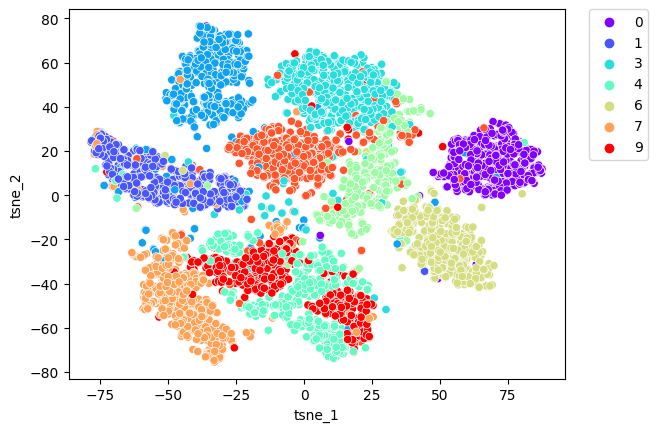
\includegraphics[width=1\linewidth]{Imagedata1/tsne.png}
	\caption{ Διάγραμμα απεικονισμού κλάσεων }
	\label{f:g1}	
\end{figure}

\clearpage

\subsection{Spectral clustering with rbf}

Στο συγκεκριμένο αλγόριθμο ο αριθμός των clusters να ήταν δέκα και το rbf επιλέχθηκε ώς δείκτης ομοιότητας μεταξύ των σημείων των δεδομένων.
Το αποτέλεσμα αυτού του αλγορίθμου φάνηκε σε δύο μετρικές, στην μετρική της ομοιογένειας και της σιλουέτας. To Silhouette score: $-0.405$ και το Homogeneity score: $0.246$, τα οποιά είναι πολύ χαμηλά, κάτι που φαίνεται και στο διάγραμμα \ref{f:g2}.

\begin{figure}[ht]
	\centering
	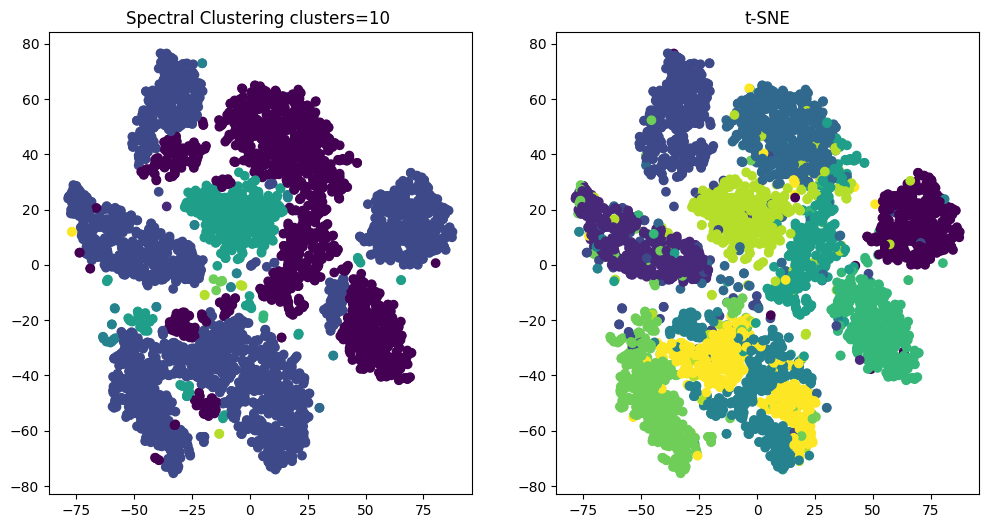
\includegraphics[width=1\linewidth]{Imagedata1/rbftsne.png}
	\caption{ Διαγράμματα σύγκρισεις απεικόνισης κλάσεων }
	\label{f:g2}	
\end{figure}

\clearpage

\subsection{Spectral clustering with nearest neighbors}

Στην συνέχεια αναπτύχθηκε ο ίδιος αλγόριθμος με διαφορετικό δείκτη ομοιότητας (affinity), ο οποίος είναι o nearest neighbors. Επιλέχθηκε να αλλάζει ο αριθμός των cluster και ο αριθμός των γειτόνων απο το 5 μέχρι το 40 με βήμα 5. Τα αποτελέσματα φάνηκαν στις δύο μετρικές στον πίνακα \ref{tab:abc}. Το καλύτερο αποτέλεσμα για την πρώτη μετρική δίνεται όταν οι γείτονες και oι cluster είναι 15 \ref{f:g3}, και για την δεύτερη όταν είναι 35 \ref{f:g4}.

\begin{table}[ht]
	\centering
	\caption{Μετρικές για διαφορετικές τιμές cluster/γειτόνων}
	\begin{tabular}{l | l | l}
		Τιμή cluster/γειτόνων & Silhouette score &  Homogeneity score\\
		\hline
		5 & -0.158 & 0.192\\
		10 & 0.443 & 0.728\\
		15 & 0.428&0.785\\
		20 & 0.389 & 0.789\\
		25 &0.369 & 0.793\\
		30 & 0.354 & 0.799\\
		35 & 0.360 & 0.820\\
	\end{tabular}
	
	\label{tab:abc}
\end{table}
\begin{figure}[ht]
	\centering
	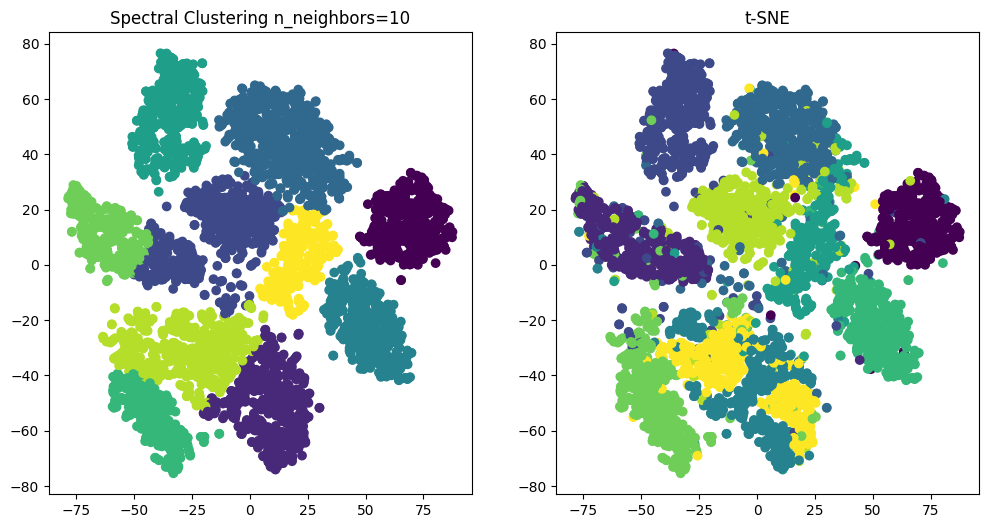
\includegraphics[width=1\linewidth]{Imagedata1/n_15tsne.png}
	\caption{ Διαγράμματα σύγκρισεις απεικόνισης κλάσεων }
	\label{f:g3}	
\end{figure}
\begin{figure}[ht]
	\centering
	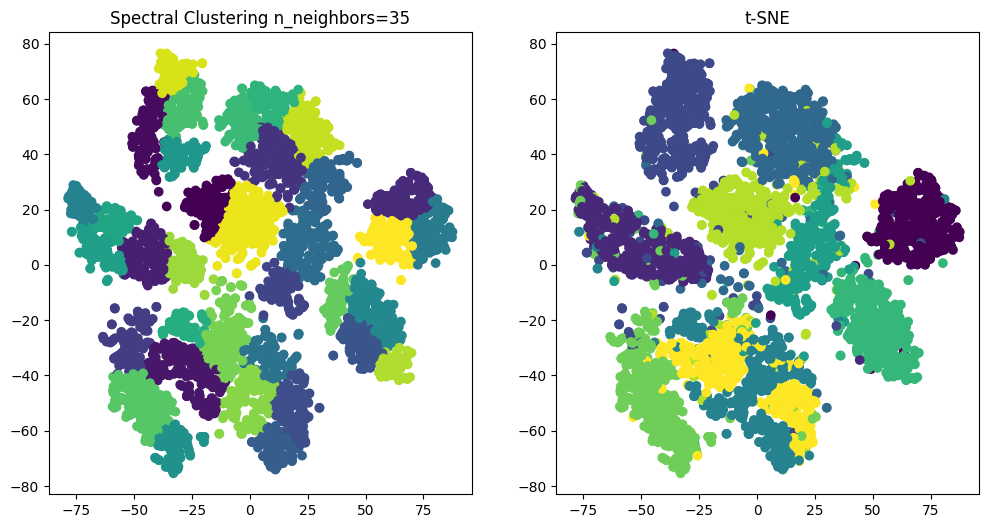
\includegraphics[width=1\linewidth]{Imagedata1/n_35tsne.png}
	\caption{ Διαγράμματα σύγκρισεις απεικόνισης κλάσεων }
	\label{f:g4}	
\end{figure}
\subsection{Kmeans}
Ακόμη χρησιμοποιήθηκε ο αλγόριθμος Kmeans, στον οποίο ελέγχθηκαν οι ίδιες μετρικές με πρίν για διαφορετικό αριθμο clusters, από 2 μέχρι 28 με βήμα 5. Τα αποτελέσματα φαίνονται στον πίνακα \ref{tab:abc1} παρακάτω. Το καλύτερο αποτέλεσμα για την πρώτη μετρική δίνεται όταν oι cluster είναι 12 \ref{f:g5}, και για την δεύτερη όταν είναι 27 \ref{f:g6}.

\begin{table}[ht]
	\centering
	\caption{Μετρικές για διαφορετικές τιμές cluster}
	\begin{tabular}{l | l | l}
		Τιμή cluster & Silhouette score &  Homogeneity score\\
		\hline
		2 & 0.378 & 0.244\\
		7 & 0.436 & 0.616\\
		12 & 0.457&0.766\\
		17 & 0.411 & 0.775\\
		22 &0.405 & 0.796\\
		27 & 0.401 & 0.797\\
	\end{tabular}
	
	\label{tab:abc1}
\end{table}
\begin{figure}[ht]
	\centering
	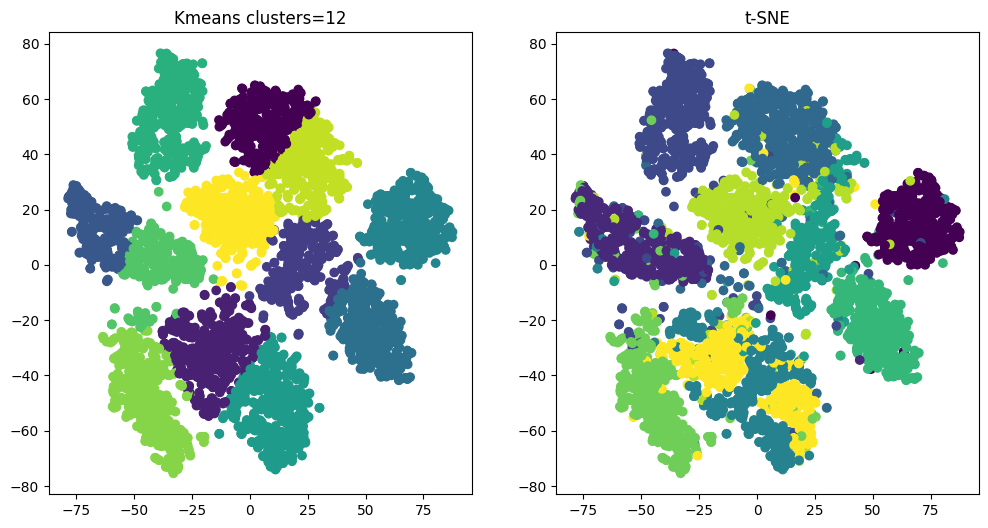
\includegraphics[width=1\linewidth]{Imagedata1/k_12tsne.png}
	\caption{ Διαγράμματα σύγκρισεις απεικόνισης κλάσεων }
	\label{f:g5}	
\end{figure}
\begin{figure}[ht]
	\centering
	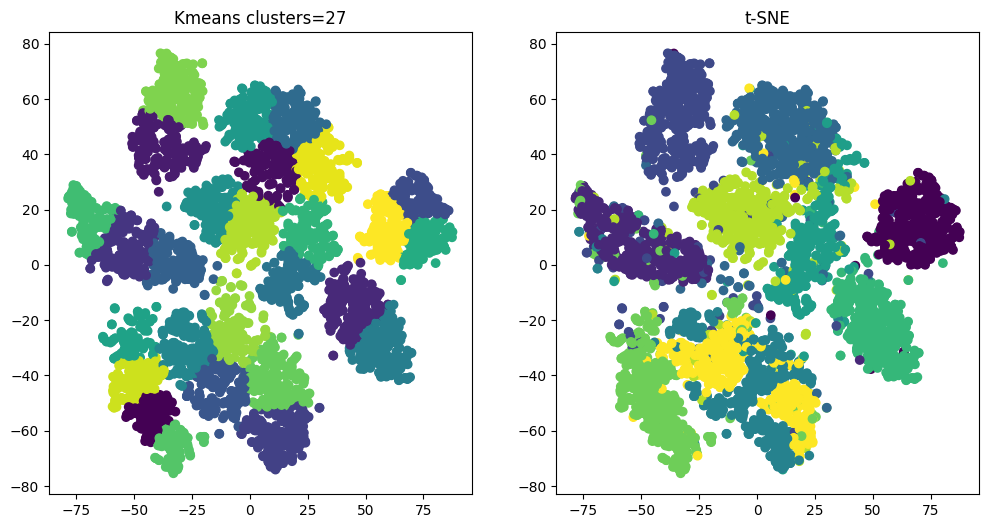
\includegraphics[width=1\linewidth]{Imagedata1/k_27tsne.png}
	\caption{ Διαγράμματα σύγκρισεις απεικόνισης κλάσεων }
	\label{f:g6}	
\end{figure}
\clearpage

\subsection{Σύγκριση μεταξύ αλγορίθμων}
Τα αποτελεσμάτα των μετρικών είναι παρόμοια στο spectral clustering με nearest neighbors με τα αντίστοιχα του αλγορίθμου kmeans, αλλά για rbf δείκτη , τα σκόρ είναι πολύ χαμηλά.
\clearpage
\section{Isomap}
Στην συνέχεια αναπτύχθηκε ο αλγόριθμος Isomap για την μέιωση των διαστάσεων σε δύο στο dataset. Ελέγχθηκαν διαφορετικές τιμές components στο isomap και όλες βγάλανε παρόμοια αποτελέσματα στις απεικονίσεις των διαγραμμάτων, για αυτό τον λόγο η διερέυνηση των αλγορίθμων Spectral clustering και kmeans έγινε με components = 10 στο Isomap




\subsection{Spectral clustering with nearest neighbors}

Στην συνέχεια αναπτύχθηκε ο ίδιος αλγόριθμος με διαφορετικό δείκτη ομοιότητας (affinity), ο οποίος είναι o nearest neighbors. Επιλέχθηκε να αλλάζει ο αριθμός των cluster και ο αριθμός των γειτόνων απο το 5 μέχρι το 40 με βήμα 5. Τα αποτελέσματα φάνηκαν στις δύο μετρικές στον πίνακα \ref{tab:abc3}. Το καλύτερο αποτέλεσμα και για τις δύο μετρικές δίνεται όταν οι clusters και οι γείτονες είναι 30 \ref{f:g7}.

\begin{table}[ht]
	\centering
	\caption{Μετρικές για διαφορετικές τιμές cluster/γειτόνων}
	\begin{tabular}{l | l | l}
		Τιμή cluster/γειτόνων & Silhouette score &  Homogeneity score\\
		\hline
		5 & 0.228 & 0.390\\
		10 & 0.308 & 0.415\\
		15 & 0.308&0.410\\
		20 & 0.322 & 0.420\\
		25 &0.322 & 0.421\\
		30 & 0.323 & 0.421\\
		35 & 0.322 & 0.421\\
	\end{tabular}
	
	\label{tab:abc3}
\end{table}
\begin{figure}[ht]
	\centering
	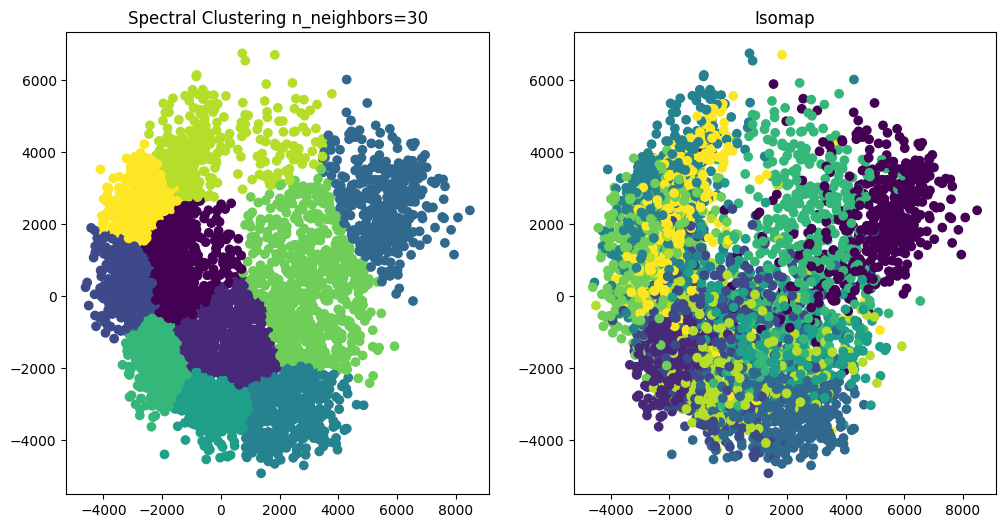
\includegraphics[width=1\linewidth]{Imagedata1/n_30isomap.png}
	\caption{ Διαγράμματα σύγκρισεις απεικόνισης κλάσεων }
	\label{f:g7}	
\end{figure}

\subsection{Kmeans}
Ακόμη χρησιμοποιήθηκε ο αλγόριθμος Kmeans, στον οποίο ελέγχθηκαν οι ίδιες μετρικές με πρίν για διαφορετικό αριθμο clusters, από 2 μέχρι 28 με βήμα 5. Τα αποτελέσματα φαίνονται στον πίνακα \ref{tab:abc2} παρακάτω. Το καλύτερο αποτέλεσμα για την πρώτη μετρική δίνεται όταν oι cluster είναι 2 \ref{f:g8}, και για την δεύτερη όταν είναι 27 \ref{f:g9}.

\begin{table}[ht]
	\centering
	\caption{Μετρικές για διαφορετικές τιμές cluster}
	\begin{tabular}{l | l | l}
		Τιμή cluster & Silhouette score &  Homogeneity score\\
		\hline
		2 & 0.441 & 0.173\\
		7 & 0.369 & 0.374\\
		12 & 0.380&0.432\\
		17 & 0.372 & 0.451\\
		22 &0.352 & 0.472\\
		27 & 0.341 & 0.479\\
	\end{tabular}
	
	\label{tab:abc2}
\end{table}
\begin{figure}[ht]
	\centering
	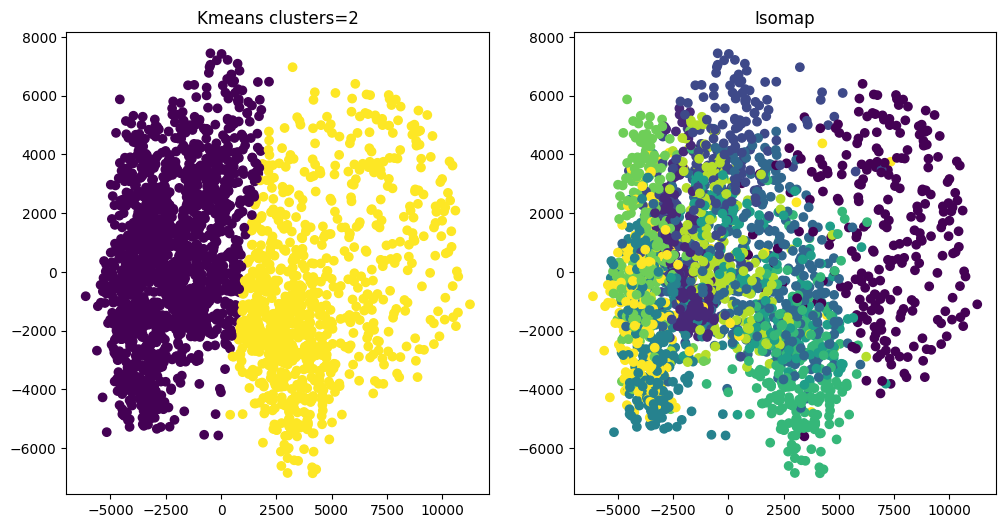
\includegraphics[width=1\linewidth]{Imagedata1/k_2isomap.png}
	\caption{ Διαγράμματα σύγκρισεις απεικόνισης κλάσεων }
	\label{f:g8}	
\end{figure}
\begin{figure}[ht]
	\centering
	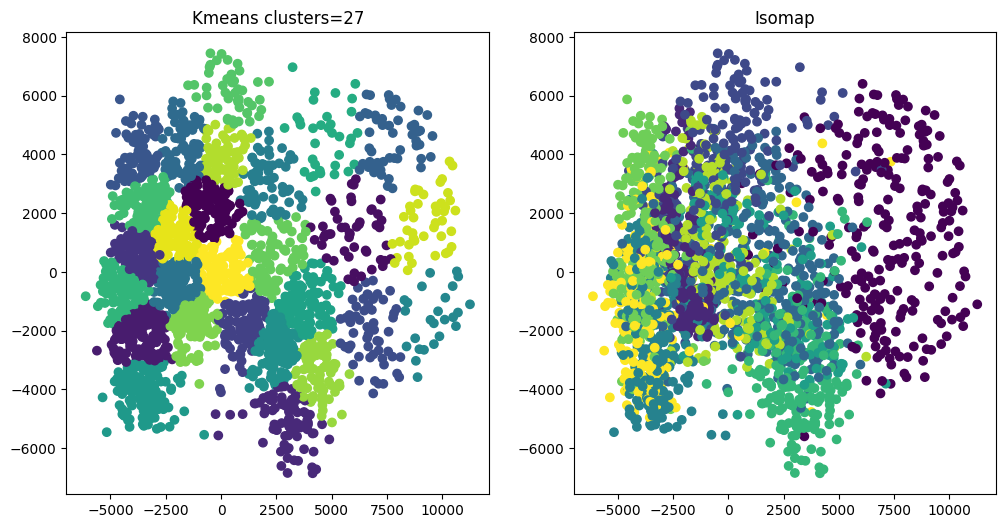
\includegraphics[width=1\linewidth]{Imagedata1/k_27isomap.png}
	\caption{ Διαγράμματα σύγκρισεις απεικόνισης κλάσεων }
	\label{f:g9}	
\end{figure}
\clearpage

\subsection{Σύγκριση μεταξύ αλγορίθμων}
Τα αποτελεσμάτα των μετρικών είναι παρόμοια στο spectral clustering με nearest neighbors με τα αντίστοιχα του αλγορίθμου kmeans. Στο πρώτο η διαφορές μεταξύ των βημάτων είναι μικρές στις μετρικές.

\clearpage

\section{Σύγκριση μεταξύ t-SNE και Isomap}
Παρατηρείται μεγάλη διαφορά στα αποτελέσματα των μετρικών μεταξύ των δύο αλγορίθμων μείωσης της διάστασης των δεδομένων. Συγκεκριμένα φαινεται ότι η μέθοδος t-SNE ταιριάζει περισσότερο στην MNIST digits, αφού οι clustering αλγόριθμοι δουλεύουν πιο αποτελσματικά στον διαχωρισμό των κλάσεων. Επίσης παρατηρείται ότι κανένας απο των δύο αλγορίθμους μείωσης των διαστάσεων, δεν έβγαλε ένα πολυ ικανοποιητικό αποτέλεσμα. Αυτό ίσως να φταίει στο γεγονός ότι συνήθως όταν αναπτύσσονται αλγόριθμοι σαν τον t-SNE , χρησιμοποιούνται πρίν απο αυτούς και άλλες μέθοδοι μείωσης των διαστάσεων όπως η PCA (βλέπε προηγούμενη εργασία).